\graphicspath{{Images/untetheredWalker/}}

\chapter{Miniature Untethered Underwater Walking Robot}
\label{chap:untetheredWalker}
Current soft actuators rely on additional hardware such as pumps, high voltage supplies, light generation sources and magnetic field generators for their operation. 
% Assembling these actuators results in bulky robotic systems, although the body of the soft robot itself may remain miniaturized. 
These components resist miniaturization and embedding them into small-scale soft robots is challenging. This limits the mobile applications of systems that need to be entirely untethered, especially in hyper-redundant robots, where a high number of actuators are needed. Here, we introduce miniature and untethered robots made of the soft voxel actuators (SVAs) presented in Chapter~\ref{chap:SVAs}. SVAs weighing only 100\,mg require small-footprint microcontrollers for their operation, which can be embedded within the robotic system. We have demonstrated the advantages of SVA-based systems through a hyper-redundant gripper with 32 actuators and an untethered miniature robot for underwater mobile applications. Since SVAs are electrically activated, closed-loop control of the SVA-based soft robots is easily achieved with embedded microcontrollers.
\section{\capitalisewords{Background}}

\begin{figure}[!ht]
\centering
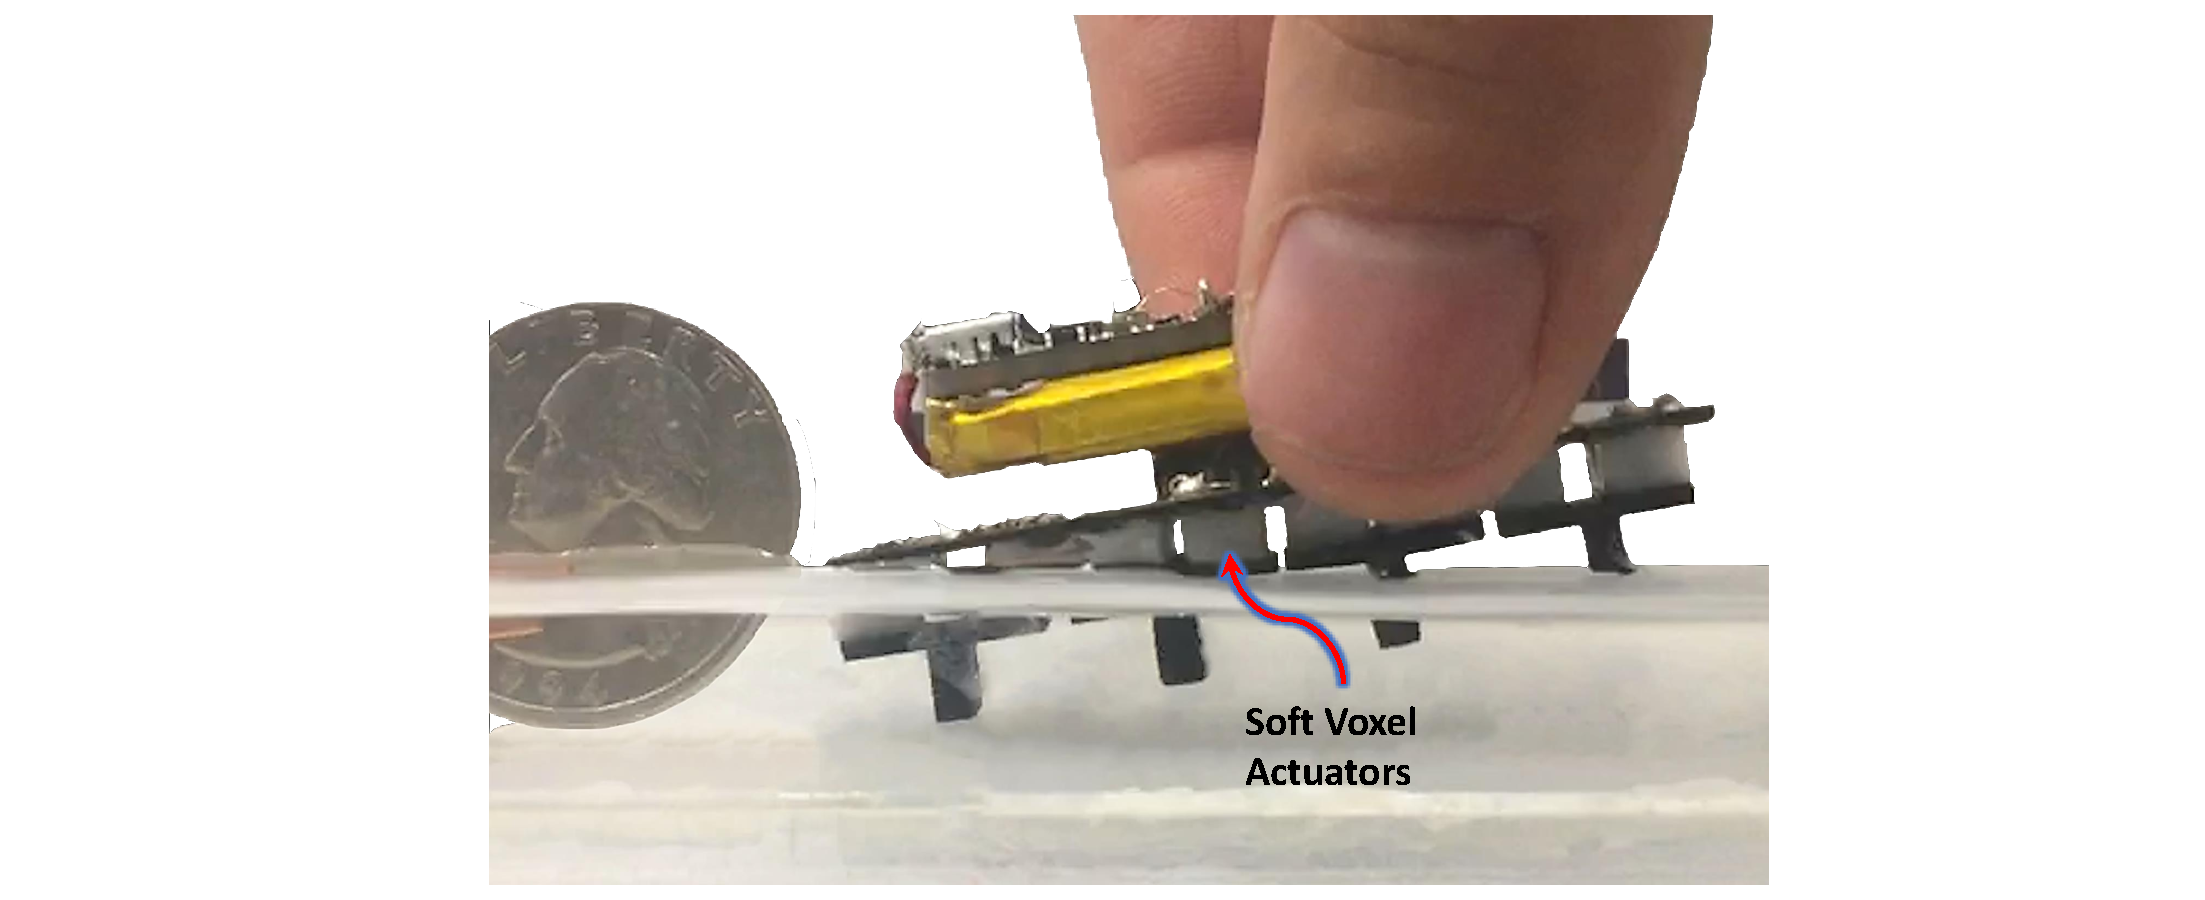
\includegraphics[width=0.6\textwidth]{untWalker.pdf}
    \caption[\capitalisewords{Untethered miniature underwater walking robot}]{An untethered miniature underwater walking robot using 8 SVAs is made which weighs only 20\,g including battery and electronics.}
    \label{fig:untWalker}
\end{figure}

Inspired by biology, soft robot developers try to utilize the advantages inherent in soft, compliant matter to achieve safer interactions around humans or more robust locomotion and manipulation in unstructured environments~\cite{martinez2013,laschi2012,tolley2014b,AdamBilodeau2015}.  
Soft pneumatic actuators (SPAs)~\cite{Gorissen2017, Branyan2018} are the most widely used category of soft robotic actuators. SPAs use passive materials like silicone and rely on rigid components such as motors and pumps that are difficult to downscale. Therefore, manufacturing small-scale soft actuators which have applications as envisioned by \cite{Hines2017} has remained a bottleneck in the development of miniaturized soft robots \cite{Majidi2019}. 

Stimuli-responsive soft materials have shown promise in solving some of these challenges \cite{Steele2018, Stuart2010,White2013}. The changes in the stress/strain distribution of these materials in response to variations in pH, temperature, electric field, magnetic field, and light results in motions such as bending, twisting, or elongation. However, the equipment needed to create variable stimuli such as structured light \cite{Palagi2016} or magnetic fields \cite{Kim2018} are still bulky and must be carried externally to the mobile system. Temperature responsive hydrogels, by contrast, can be stimulated electrically using Joule heating \cite{Yu2013}. Electrical stimulation can be confined to small regions, making it possible to create more precise motion \cite{Richter2009}. We have previously reported solving some of the challenges associated with temperature responsive poly(N-isopropylacrylamide) (PNIPAAm) based hydrogels such as slow response and tunability of mechanical properties. We have also introduced blocks called soft voxel actuators (SVAs), which are electrically activated by Joule heaters \cite{Khodambashi2021}. Here, we demonstrate how SVAs support the development of soft robots which are miniature and untethered -- two key characteristics that are challenging to realize with pneumatic soft actuators. We introduce a miniature and completely untethered robot for underwater applications; this robot, which weighs only 20\,g including its battery and electronics, can be seen in Fig.~\ref{fig:untWalker}. We also demonstrate the use of SVAs to build a miniature gripper with hyper-redundant DOFs as shown in Fig.~\ref{fig:gripper}. This gripper uses two manipulators each with 16 actuators and dimensions of $10\times 40 \times 4.5\,mm^3$. 

	
\section{\capitalisewords{Assembling the robots using SVAs}}
A voxel actuator can be made in different shapes and dimensions based on design requirements. Manufacturing a SVA is performed via a molding process in which a hydrogel precurosor solution is poured into a mold, a Joule heater is inserted into the mold and the solution is then polymerized with a UV LED. Surface mount  resistors  (10\,ohm  SMD  resistor  0805) were chosen as the heating elements. For the construction of the hyper-redundant gripper, the voxels are made as cubes of 4.5$\times$4.5$\times$4.5\,mm$^3$ as shown in Fig.~\ref{fig:gripper}. In the case of the untethered walking robot, voxels of 8$\times$4.5$\times$3\,mm$^3$ are used. Details of hydrogel synthesis, material characterization and SVA manufacturing are discussed in Chapter~\ref{chap:SVAs}.

\section{\capitalisewords{Results}}
Hydrogels expand and contract based on the diffusion of water into and out of their structure when the temperature is passed their critical transition temperature -- which is around 32\textsuperscript{o} C in case of PNIPAAm hydrogels. Therefore, all the experiments have been performed in a water bath. Fig.~\ref{fig:heterogeneous} shows a schematic of a SVA. When the embedded Joule heater is turned on, the temperature increases and the volume of the hydrogel decreases. When the heater turns off, the SVA cools down and its volume increases. We have shown that a SVA can produce a force of 0.12\,N, equivalent to nearly 12\,g or 120 times its own weight \cite{Khodambashi2021}. To demonstrate how SVAs support the development of miniature and untethered soft robots, we describe two different robotic platforms in the following sections. 

\subsection{Case Study I: Miniature Hyper-redundant Soft Gripper}
The structure shown in Fig.~\ref{fig:gripper}A was assembled using 32 SVA units. The SVAs are connected together using a 0.1 mm thick 3D printed PLA sheets. Dynamic on-demand shape changes are achieved through time-varying activation of SVAs. In this experiment, SVAs 1 thorough 8 on the right side of the left arm and on the left side of the right arm are activated leading to bending of the arms in opposite direction and closing of the gripper.
% in \subfigref{fig:4}{D}. 
Each SVA is activated with maximum voltage (3.7\,V). The demonstrated miniaturized continuum gripper with 32 degrees of freedom in a $40\times11\times5$\,mm$^3$ footprint represents the highest reported electrically-addressable number of DOFs in a soft manipulator of these dimensions. 
\begin{figure*}[!ht]
      \centering
      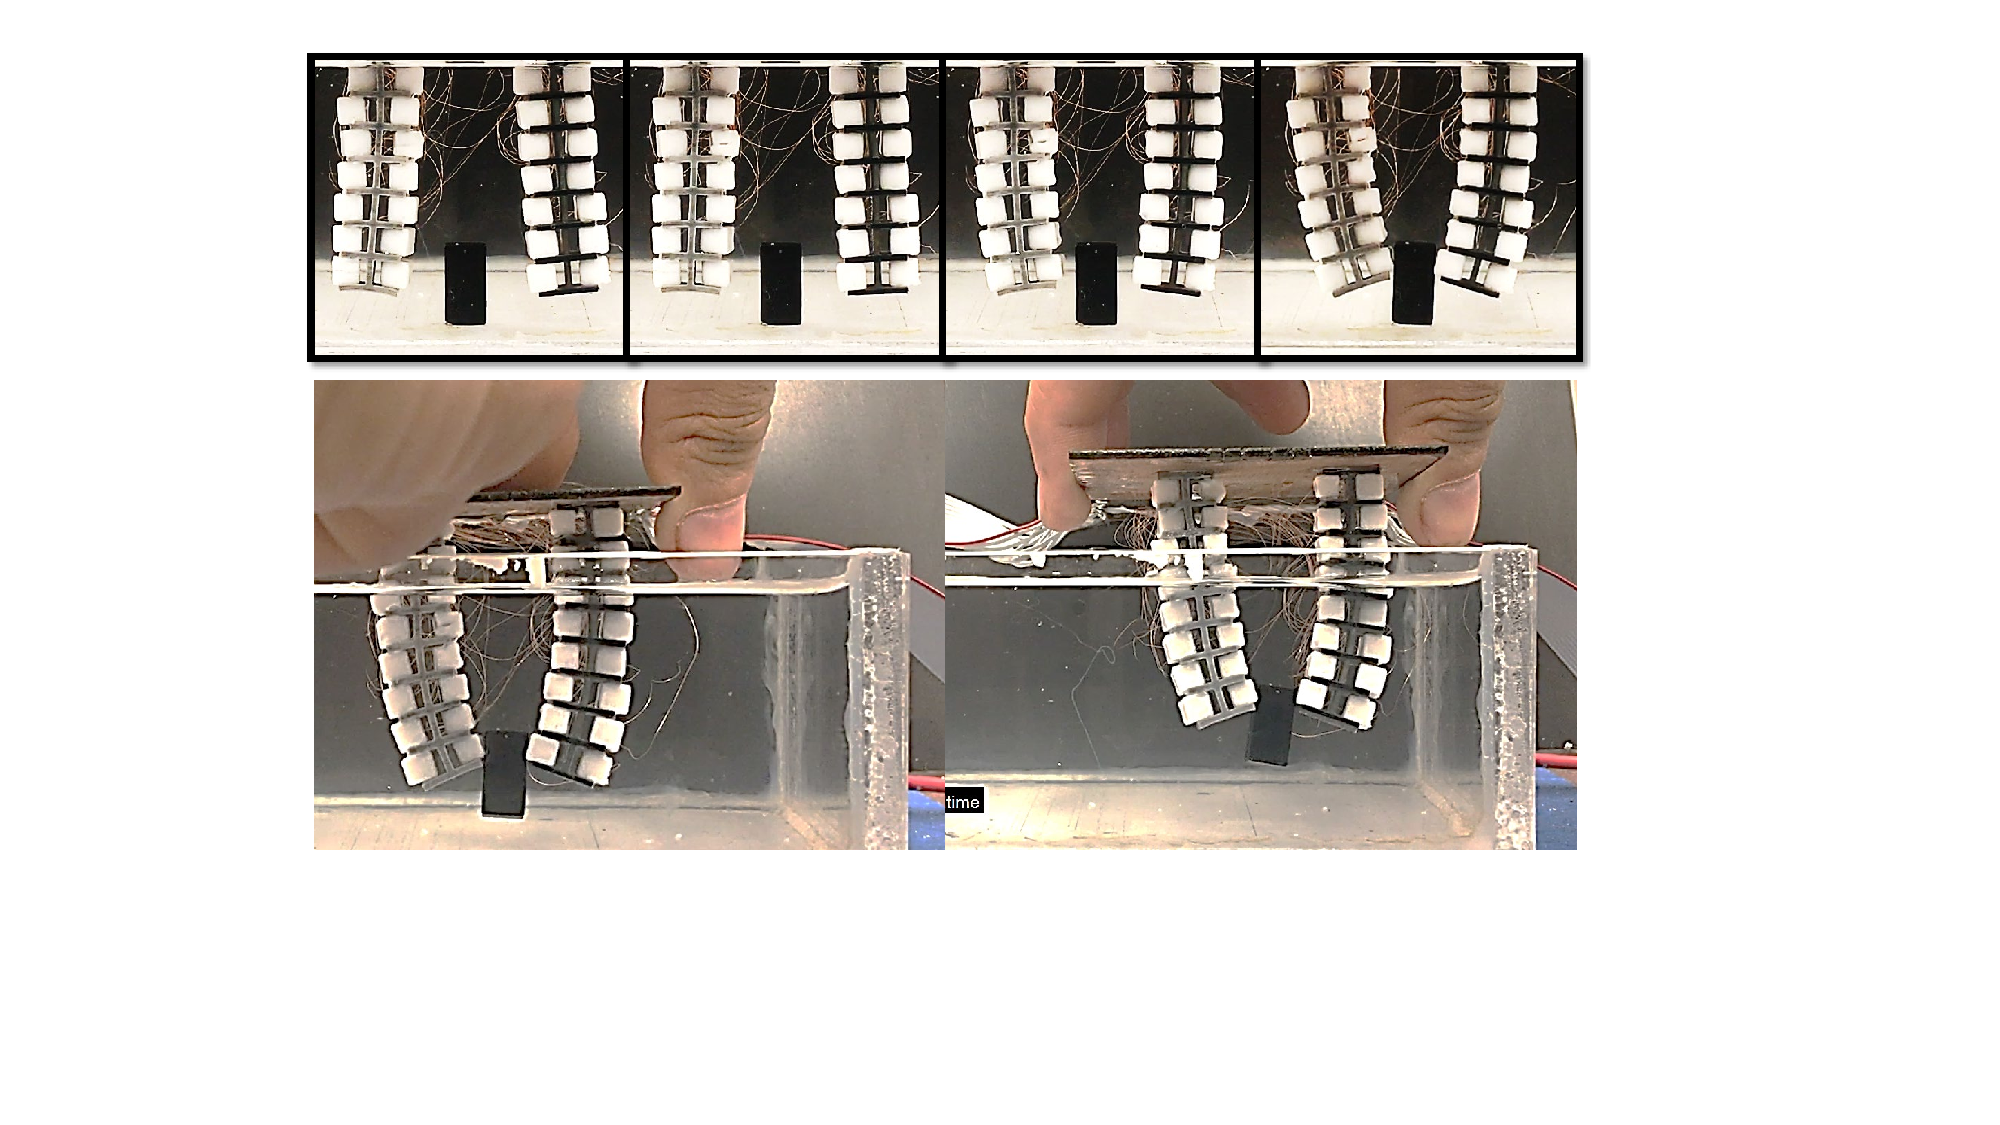
\includegraphics[width=\textwidth]{gripper.pdf}
      \caption[\capitalisewords{Hyper-redundant gripper}]{Activation of SVAs results in local increase in the temperature which leads to deformations that control the overall motion of the gripper. The gripper can produce enough force to carry a 10\,g load. }
      \label{fig:gripper}
\end{figure*}

\subsection{Case Study II: Untethered Miniature Underwater Walking Robot} 
The robot shown in Figure~\ref{fig:untWalker} has four legs. Each leg is a two-DOF manipulator composed of two SVAs and a 3D printed extension as shown in Figure~\ref{fig:untethered_podia}A. The workspace of the tip of this manipulator is plotted in Fig.~\ref{fig:untethered_podia}B. To amplify the movement of the tip and measure it more precisely, a needle is attached to the tip of the 3D printed extension. A spherical marker is attached to the end of the needle and functions as a marker for tracking using a camera (Fig.~\ref{fig:untethered_podia}C). The needle is only attached for recording the trajectories and was not present in the final robot prototype. We have created circular and oval trajectories using sine wave voltages as input to the SVAs. Each SVA is actuated using a sine wave with a phase shift with respect to other SVA. As the phase shift between the two SVAs in a manipulator is varied, the shape of the trajectory changes. Figure~\ref{fig:untethered_podia}D shows different trajectories of the tip of the needle as a function of phase shift in the sinusoidal excitation voltages. To create an untethered walking robot, four manipulators discussed above are assembled in an array. The array is attached to a microcontroller board (Adafruit Itsy Bitsy M0) and a lithium ion battery is added to the system as shown in as shown in Fig.~\ref{fig:untethered_podia}E. The movement of the miniature underwater walking robot is shown as a time-lapse in Fig.~\ref{fig:untethered_podia}F.
\begin{figure*}[!t]
      \centering
      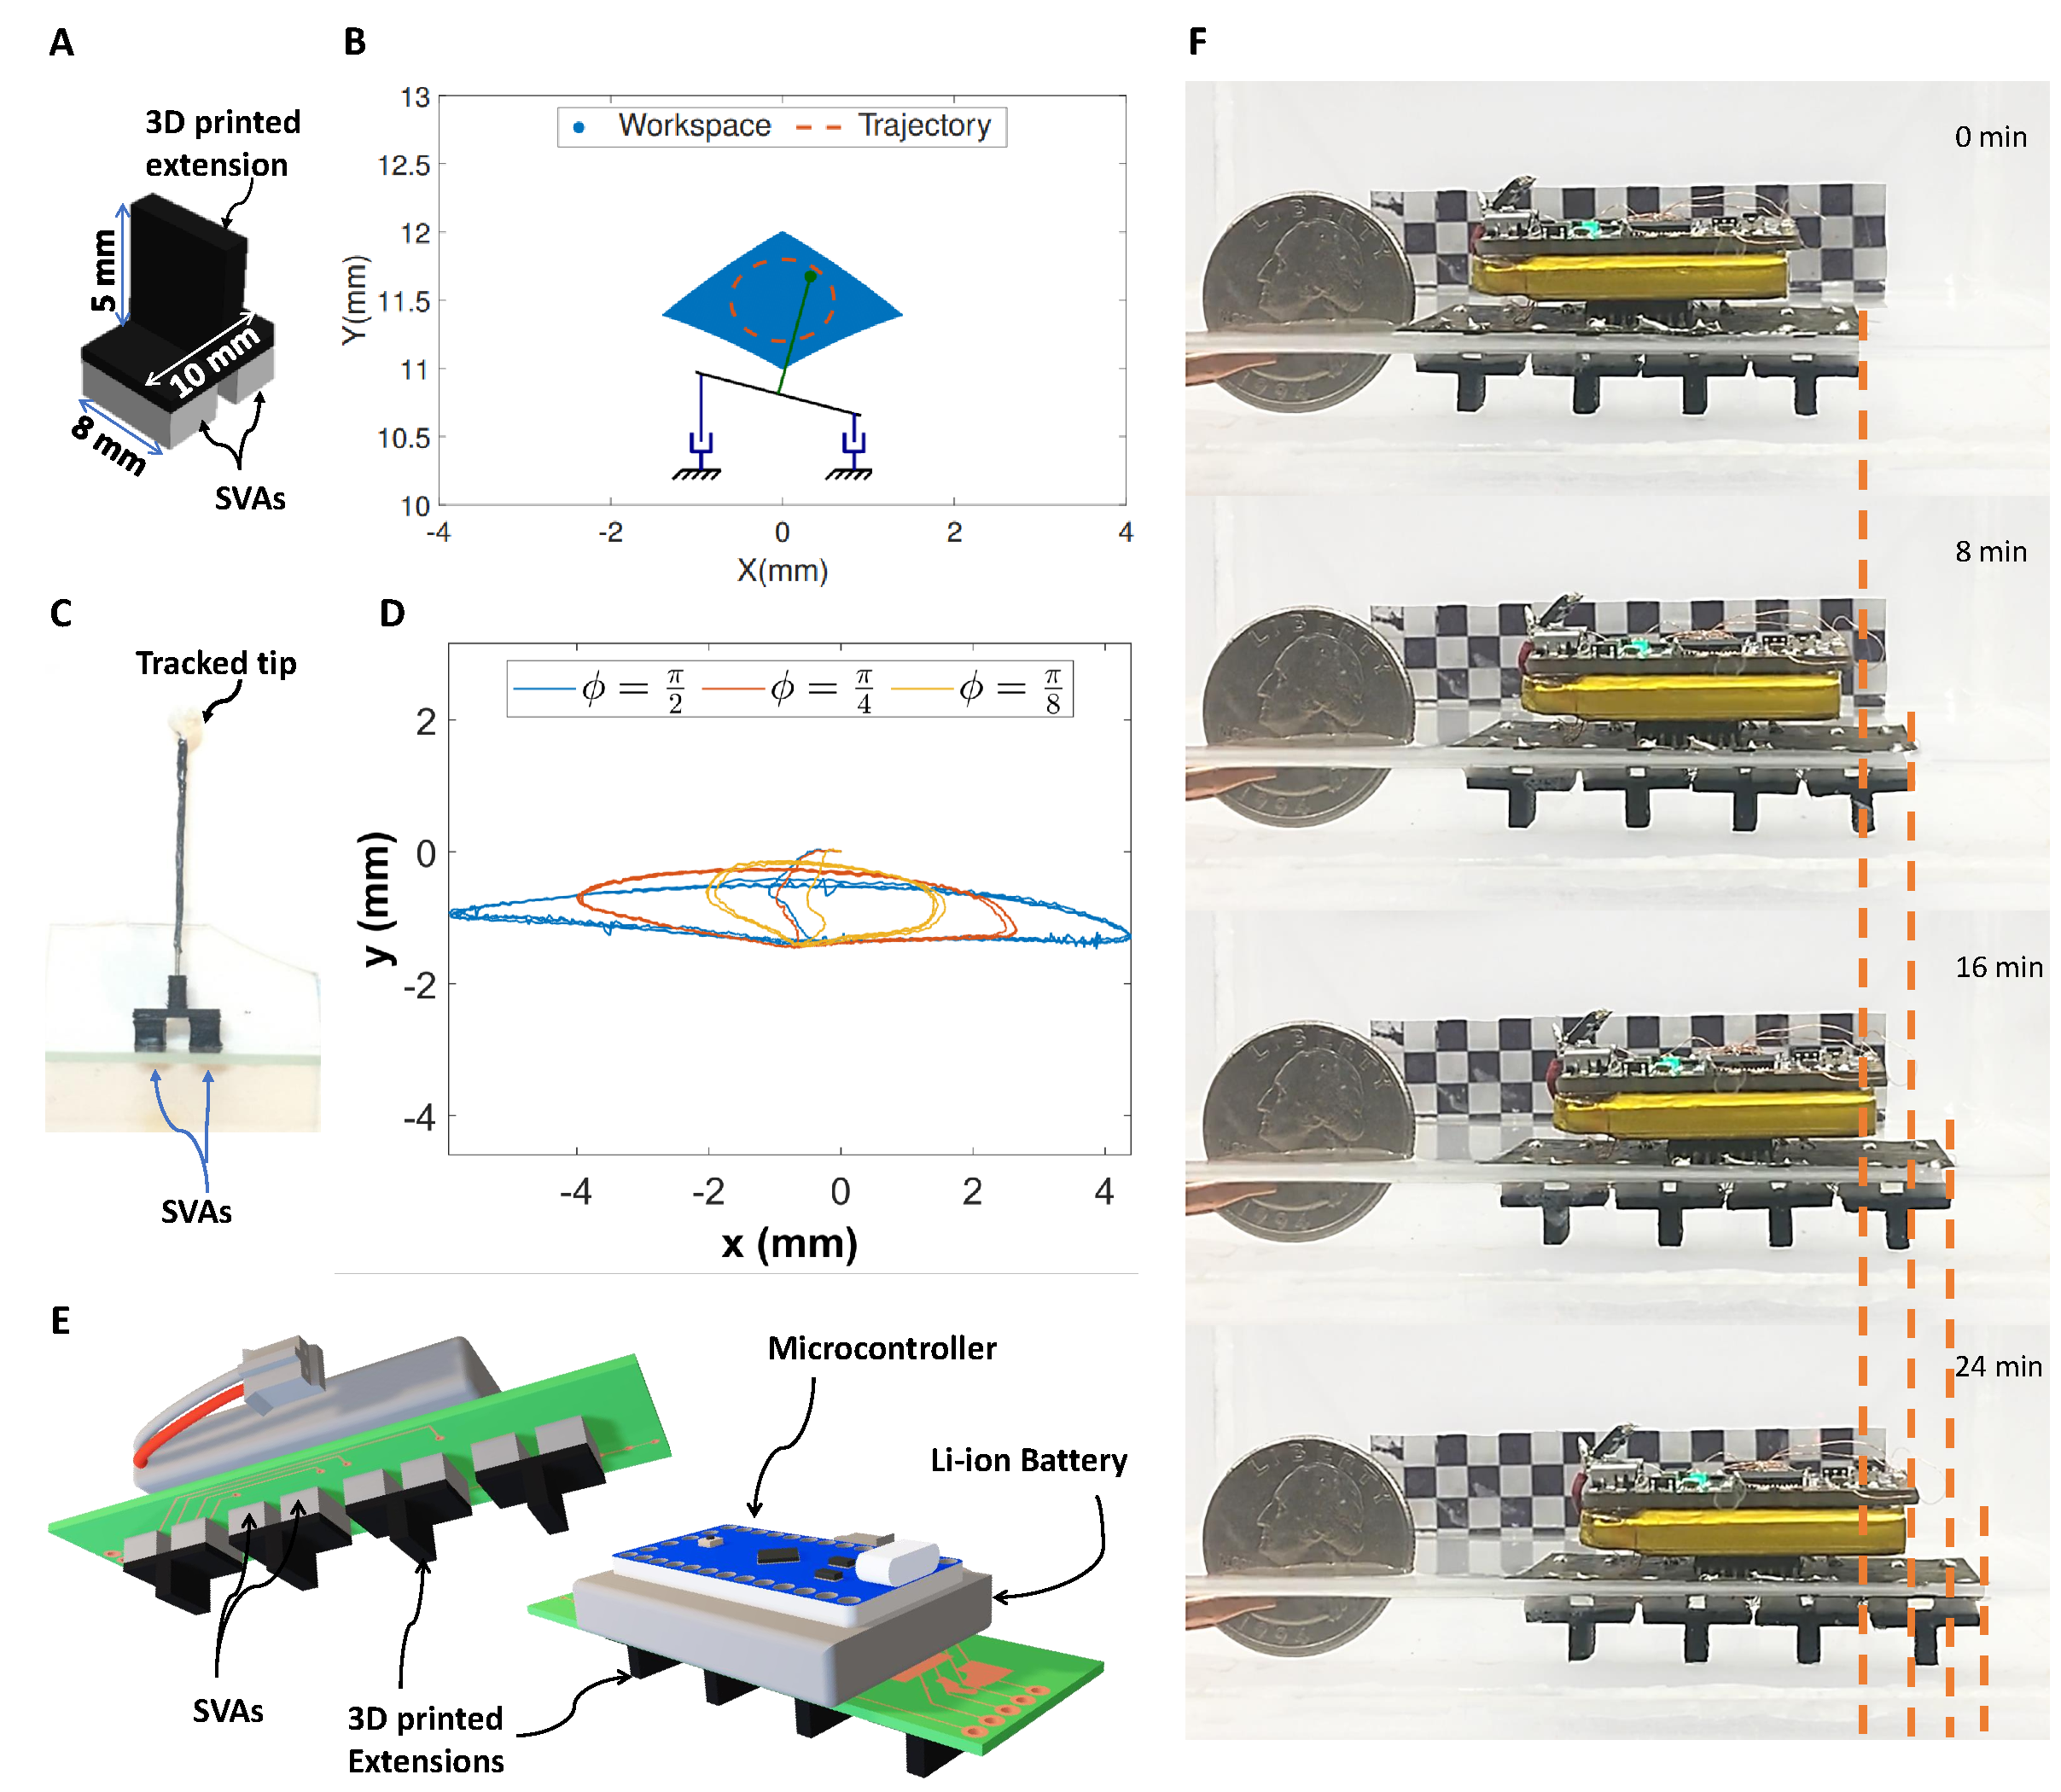
\includegraphics[width=1\textwidth]{untethered_podia.pdf}
      \caption[\capitalisewords{Design and evaluation of untethered miniature underwater walking robot}]{A) A two degrees of freedom manipulator using two SVAs and a 3D printed extension. B) The workspace of the tip of this manipulator. C) A needle is attached to the tip of the 3D printed extension to amplify the movement of the tip. D) Different trajectories of the tip of the needle as a function of phase shift in the sinusoidal excitation voltages. E) A microcontroller board and a lithium ion battery is added to the system to make an untethered robot. F) Time-lapse of the movement of the miniature underwater walking robot (see Movie S1 for details).}
      \label{fig:untethered_podia}
\end{figure*}

\subsection{Comparing Actuation of SVAs using Electrical and Light Signals}
\label{subsec:elecVSlight}
Hydrogels can be made to respond to different stimuli such as PH, Light or heat. On-demand shape changes are achieved using light as a control signal~\cite{Wang2015b}. In case of temperature responsive hydrogels such as the one presented in this work, any stimulus that can change the temperature of the gel could be used for actuation. Therefore, addition of light absorbing agents that can convert light energy to heat can result in a light responsive hydrogel. Gold nanoparticles are among the highly used light absorbing agents. Under illumination at their plasmonic resonance wavelength, they can turn incident light into efficient nano sources of heat remotely controllable by light. One such light responsive hydrogel is previously demonstrated in {Zhao, Yusen, et al. "Soft phototactic swimmer based on self-sustained hydrogel oscillator." Science Robotics 4.33 (2019).}
\begin{figure*}[!th]
      \centering
      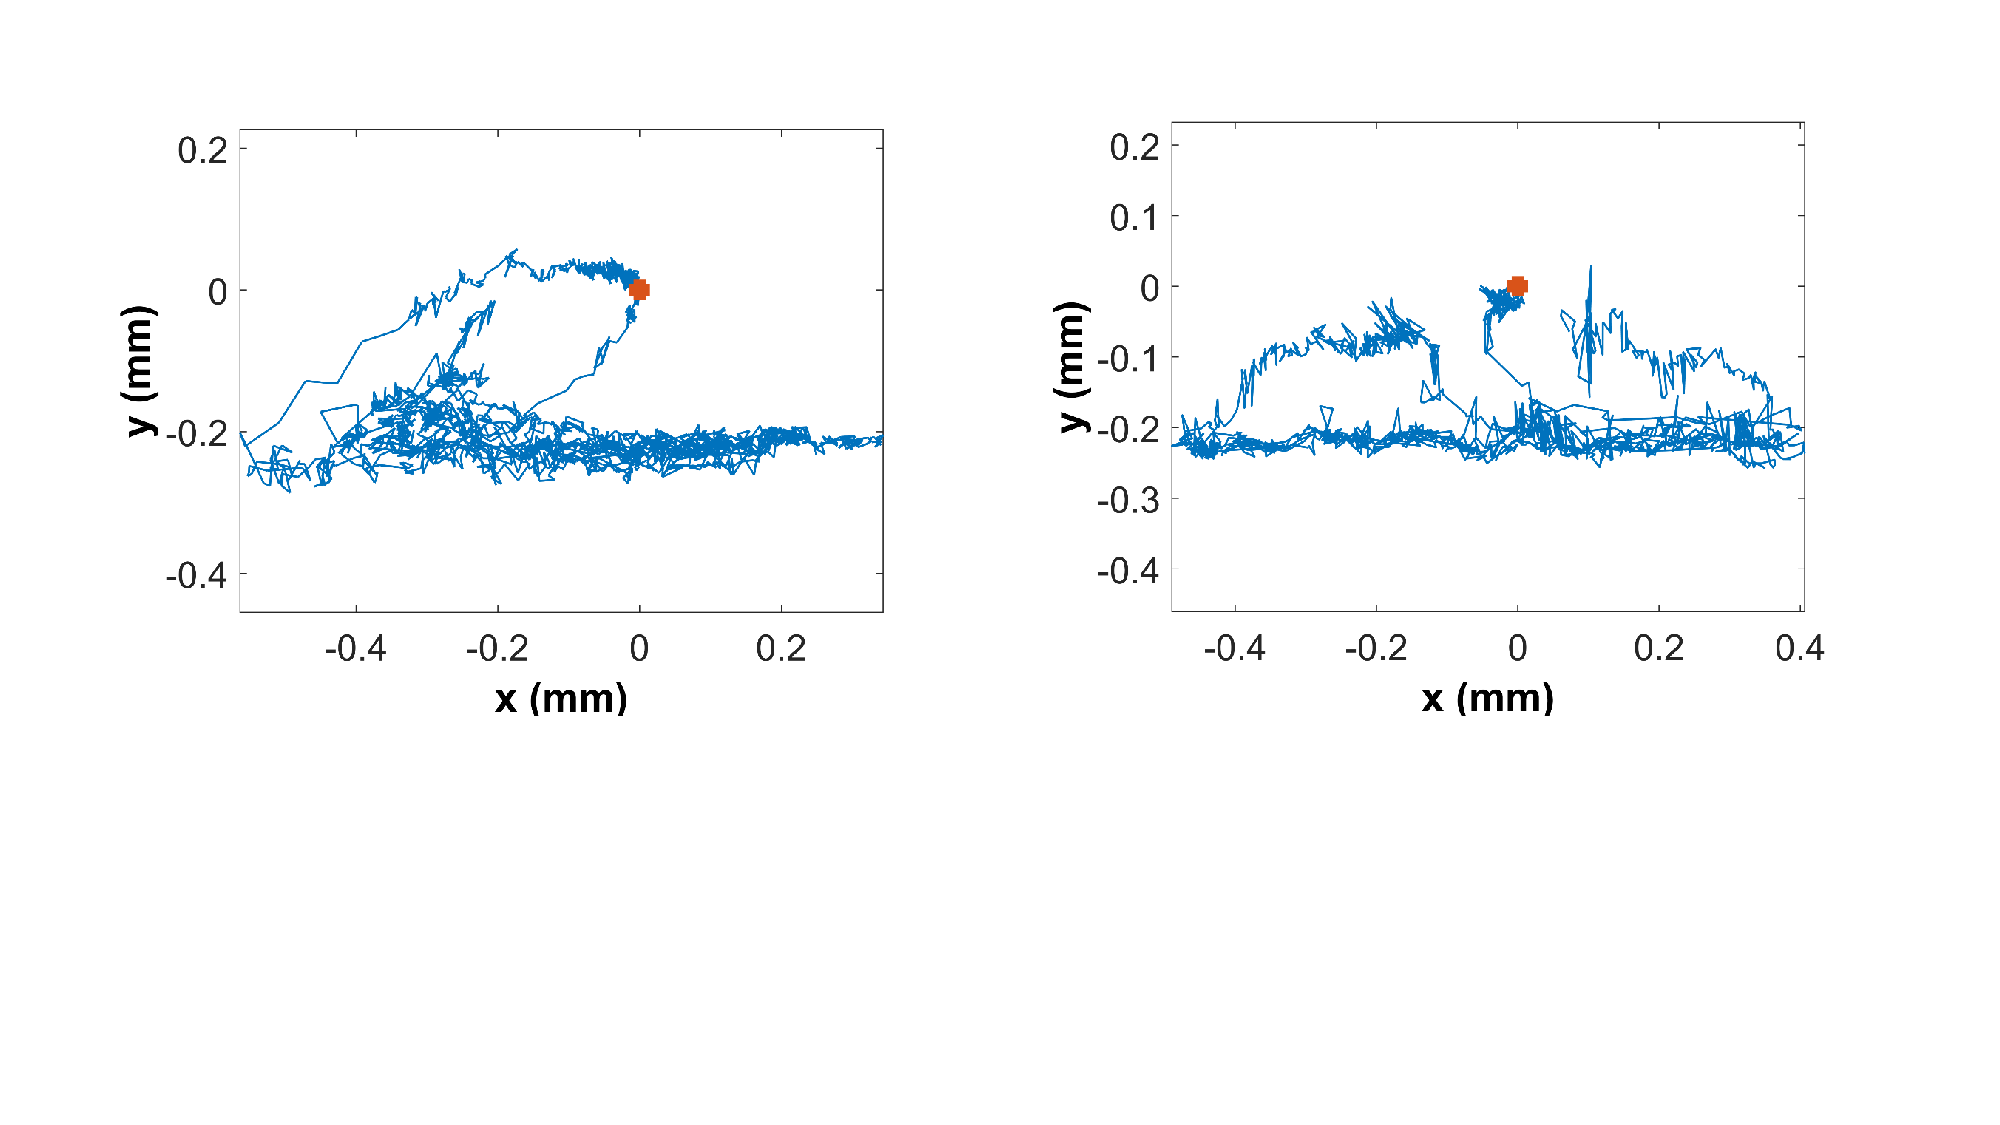
\includegraphics[width=1\textwidth]{Fig4.pdf}
      \caption[\capitalisewords{Trajectories using a light responding hydrogel}]{Trajectories produced using a light responding hydrogel. Light responding SVAs are activated using a laser source pointed manually by a human operator.}
      \label{fig:laser}
\end{figure*}
Here, to show some possibilities, polypyrrole as a light absorbing material is used to create SVAs that respond to a light beam. Using this light-responsive gel, a manipulator similar to Fig.~\ref{fig:untethered_podia}C  is built using two SVAs. As before, the goal is to move the tip of the mechanism in an oval loop. The trajectory of the tip is recorded using a camera and is shown in Figure~\ref{fig:laser}. It is clearly seen that using light as a control signal results in a random trajectory which is far from the desired one. This is because the laser beam is manually shined on the SVAs. Even if a motorized mechanism is used to shine the light, it only complicates the system making it less usable as a mobile robotic platform.  In contrast, the electric stimulation results in a much smoother trajectory that is repeatable over many cycles. It is also possible to program the desired trajectory by varying the activation voltage of SVAs. In this experiment, two sinusoidal voltages are used that have a phase shift that result in circular motion of the tip as discussed before. Animals use electric signals for activation of their muscles and the analogy of SVAs to motor units was the source of inspiration to stay with electric signals as opposed to other activation modes so that the resulting mechanisms are more independent of the environment and are more easily controlled. 

\subsection{Case Study III: Demonstration of a Closed-loop Controller Through a miniature Starfish Inspired Robot}
Up to this point, it has been shown that using electrical signals are advantageous in providing a facile method of controlling the deformation of SVAs. To show the full potential of the SVAs, a closed-loop control algorithm is implemented in a robotic platform inspired by starfish. This mechanism has the same structure as the untethered robot shown in Figure~\ref{fig:untWalker}, however instead of the two DOF manipulators touching the ground and moving the robot, the robot is stationary in an upside down configuration and manipulates an object as shown in Figure~\ref{fig:starfish}D. As shown in Figure~\ref{fig:starfish}A-C, a circuit board, which serves as the fixed base of the manipulator, is attached to one side of the two SVAs; the 3D printed T-shaped extension is attached to the other side. The circuit board and extension are attached to the SVAs with superglue to ensure that they remain in contact with the SVAs during the experiments. Since hydrogels must be immersed in water to absorb water when cooling, all experiments are conducted in a tank of deionized (DI), room-temperature water.

\begin{figure*}[!th]
      \centering
      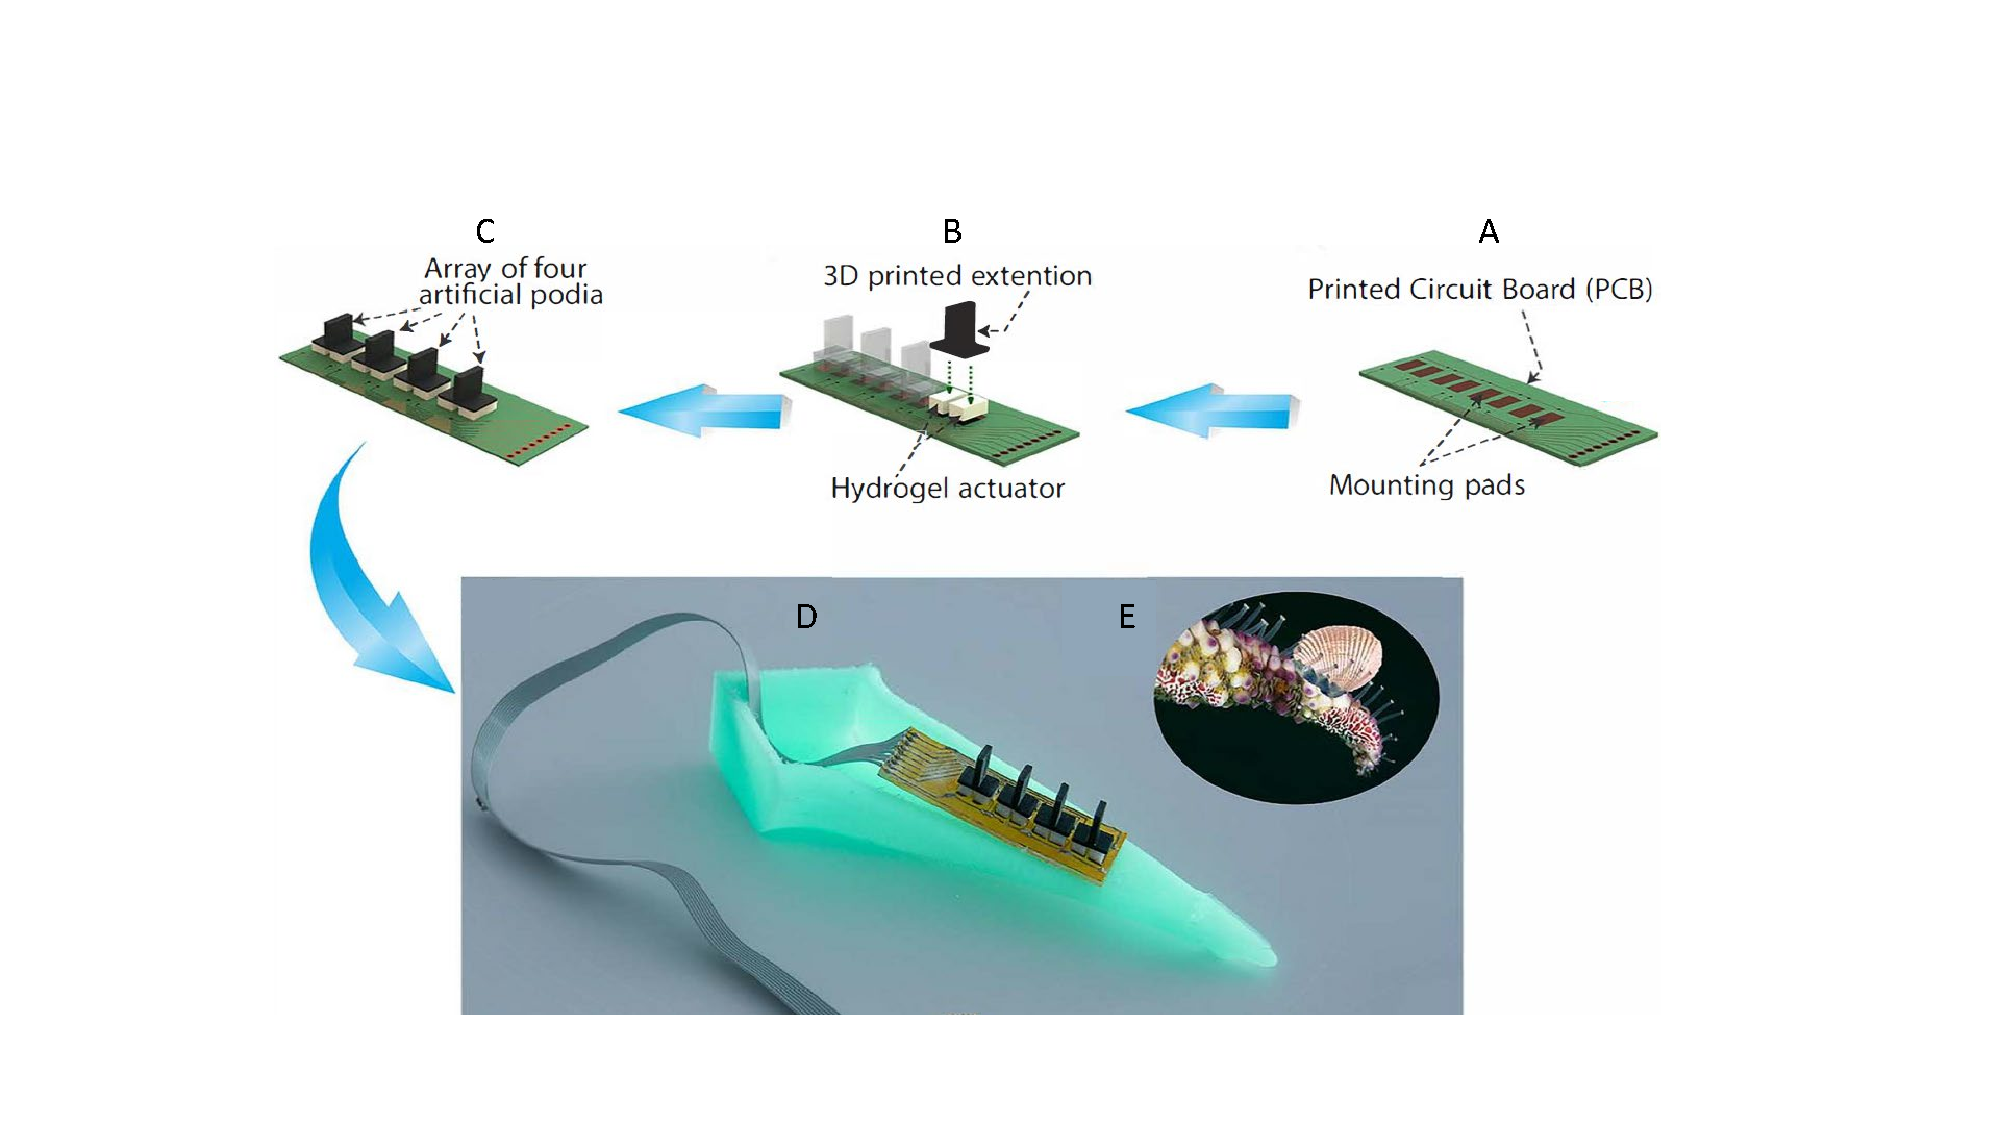
\includegraphics[width=1\textwidth]{starfish.pdf}
      \caption[\capitalisewords{A starfish inspired minature robot}]{A-C) Steps for assembling SVAs into printed circuit board and adding 3D printed podia. D) The completed prototype E) A starfish transporting food (a clam) towards its mouth.}
      \label{fig:starfish}
\end{figure*}


\begin{figure*}[!th]
      \centering
      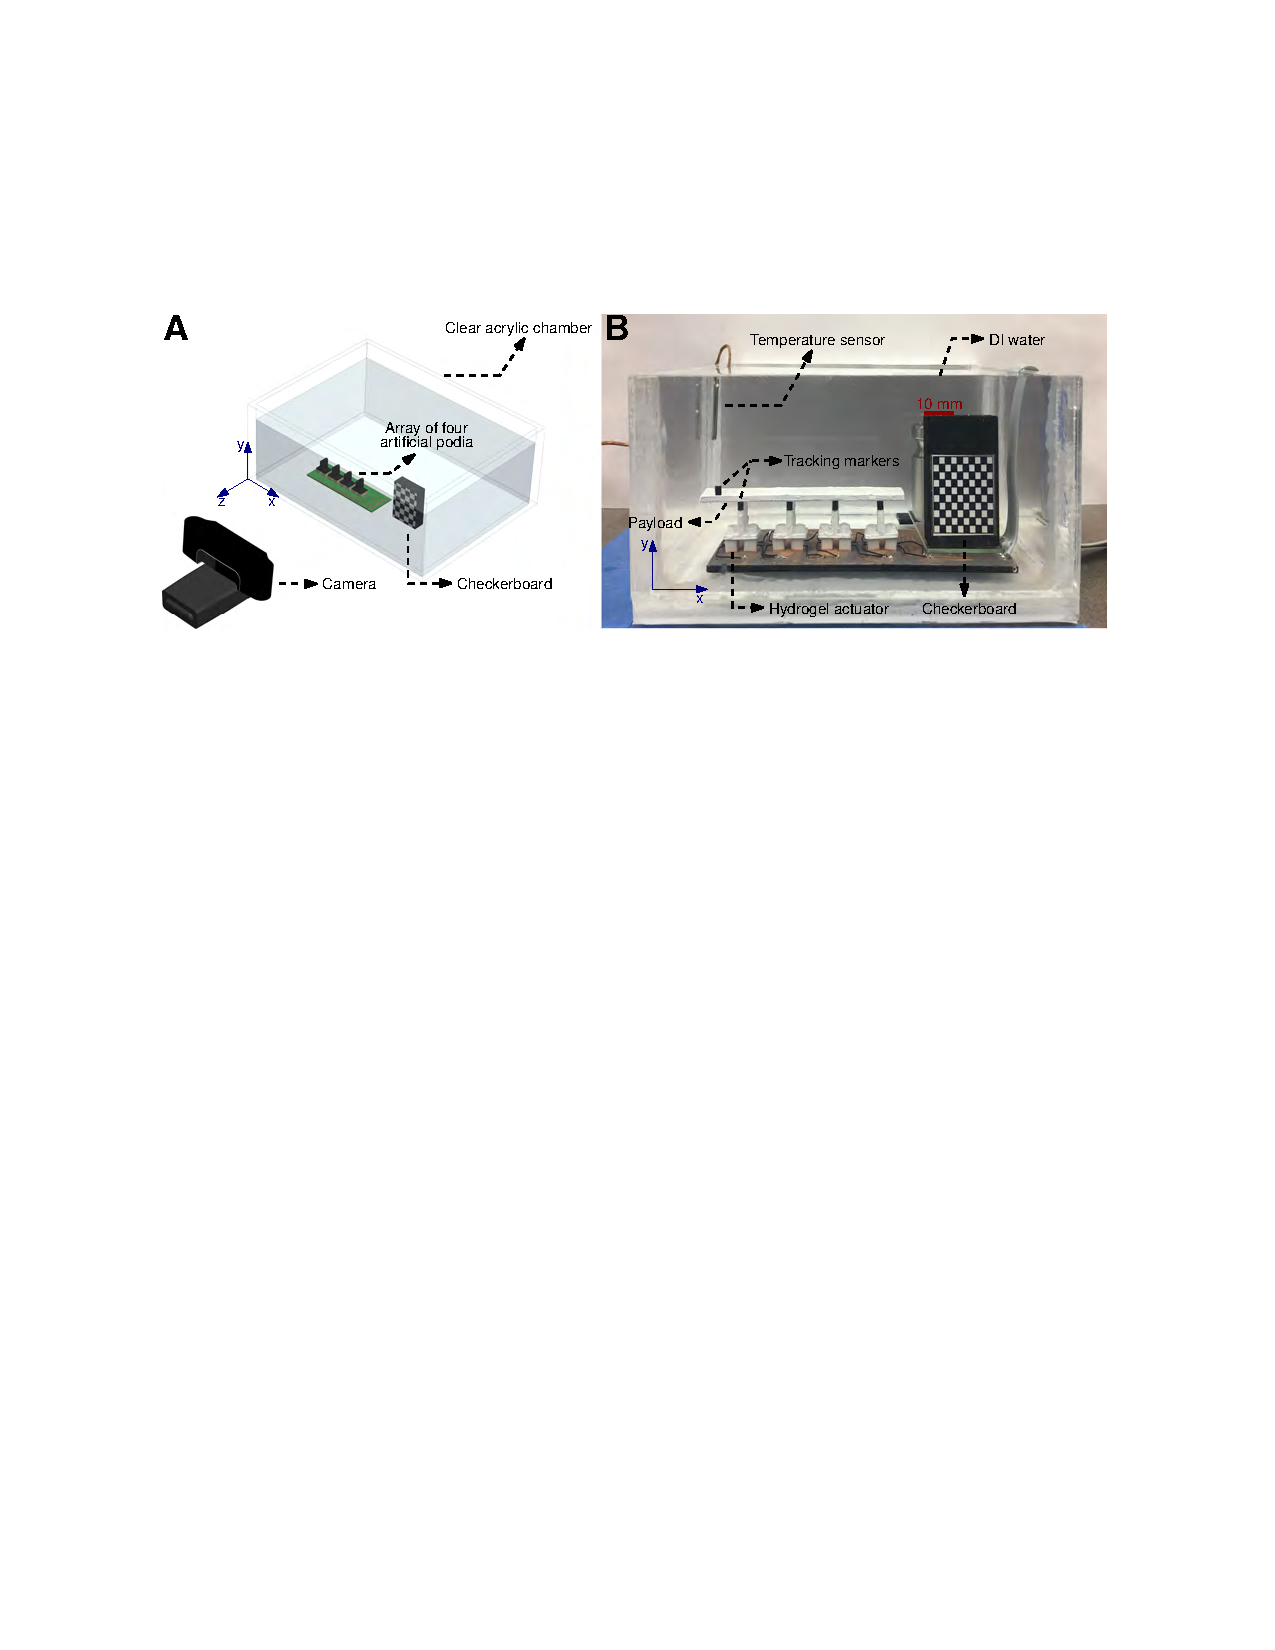
\includegraphics[width=1\textwidth]{setupCheckerboard.pdf}
      \caption[\capitalisewords{Trajectories using a light responding hydrogel}]{Trajectories produced using a light responding hydrogel. Light responding SVAs are activated using a laser source pointed manually by a human operator.}
      \label{fig:setupCheckerboard}
\end{figure*}

\subsubsection{Experimental Setup}
In a starfish, the podia moves in a loop and creates the desired motion for manipulation and locomotion. In Section ~\ref{subsec:elecVSlight} it is shown that creating a loop is possible through the use of sinusoidal signals. However, using predefined signals limits the movement to a certain pattern. For creating different motions to fit the requirements of different tasks, it is necessary to be able to control the movement of the arm on-demand based on a feedback from the environment. For this purpose, using a camera, the position of the tip of the podia is tracked and used as feedback in the control algorithm. The experiment setup is shown in Figure~\ref{fig:setupCheckerboard}A. For calibrating the camera, a checkerboard is used and the entire experiment is performed in a warer tank as illustrated in Figure~\ref{fig:setupCheckerboard}B. A Logitech C930e USB Webcam is placed in front of the tank to send real-time data to the image processing program in MATLAB which tracks the position of a marker on the manipulator tip. These measurements of the manipulator tip's position over time are transmitted back to the controller. We used a black-and-white checkerboard with 2~mm $\times$ 2~mm squares to estimate the camera calibration factors (mm/pixel) along the $x$ and $y$ axis (Figure~\ref{fig:setupCheckerboard}). White was selected as the color of the tank's background, and black was selected as the color of the manipulator tip's marker to facilitate contrast-based filtering between the foreground and background. The Camera Calibration Toolbox in MATLAB was initially used to compensate for lens distortion, but since this increased the image processing time by 30\% without significantly improving the image data, the original camera images were subsequently used without compensation. All control algorithms are implemented in MATLAB; the controller output is sent to an Arduino Mega2560, which acts as the physical communication layer between MATLAB and a  PCA9685 MOSFET board. This MOSFET board, with 16 discrete output channels, receives a PWM signal from the controller and applies it (maximum: 3.7\,V) at higher current to the corresponding Joule heater.


\subsubsection{Experimental validation of controller}
The details of the system modeling, identification, controller design and performance are discussed in Appendix~\ref{chap:control}. Here, only the results related to experimental validation of the controller is presented. Since the $H_\infty$-optimal controller exhibited higher tracking accuracy in simulation both with and without disturbance and noise (Figure~\ref{fig:sim}), it was selected for experimental implementation. Using the designed control gain for $H_\infty$, we have implemented the output-feedback tracking framework depicted in Fig.~\ref{fig:control_block}b on the hydrogel-based manipulator (Fig.~\ref{fig:setup}). Half-ellipse and quarter-ellipse paths were also used as reference trajectories. Sources of noise in the experiment arise in the testing environment and vision-based feedback. Disturbances include modeling and manufacturing errors. The MAE and NMAE values are reported for one cycle per trajectory in Table~\ref{table:control}, though three repeating cycles per trajectory were collected.

\begin{figure*}[t]
\centering
    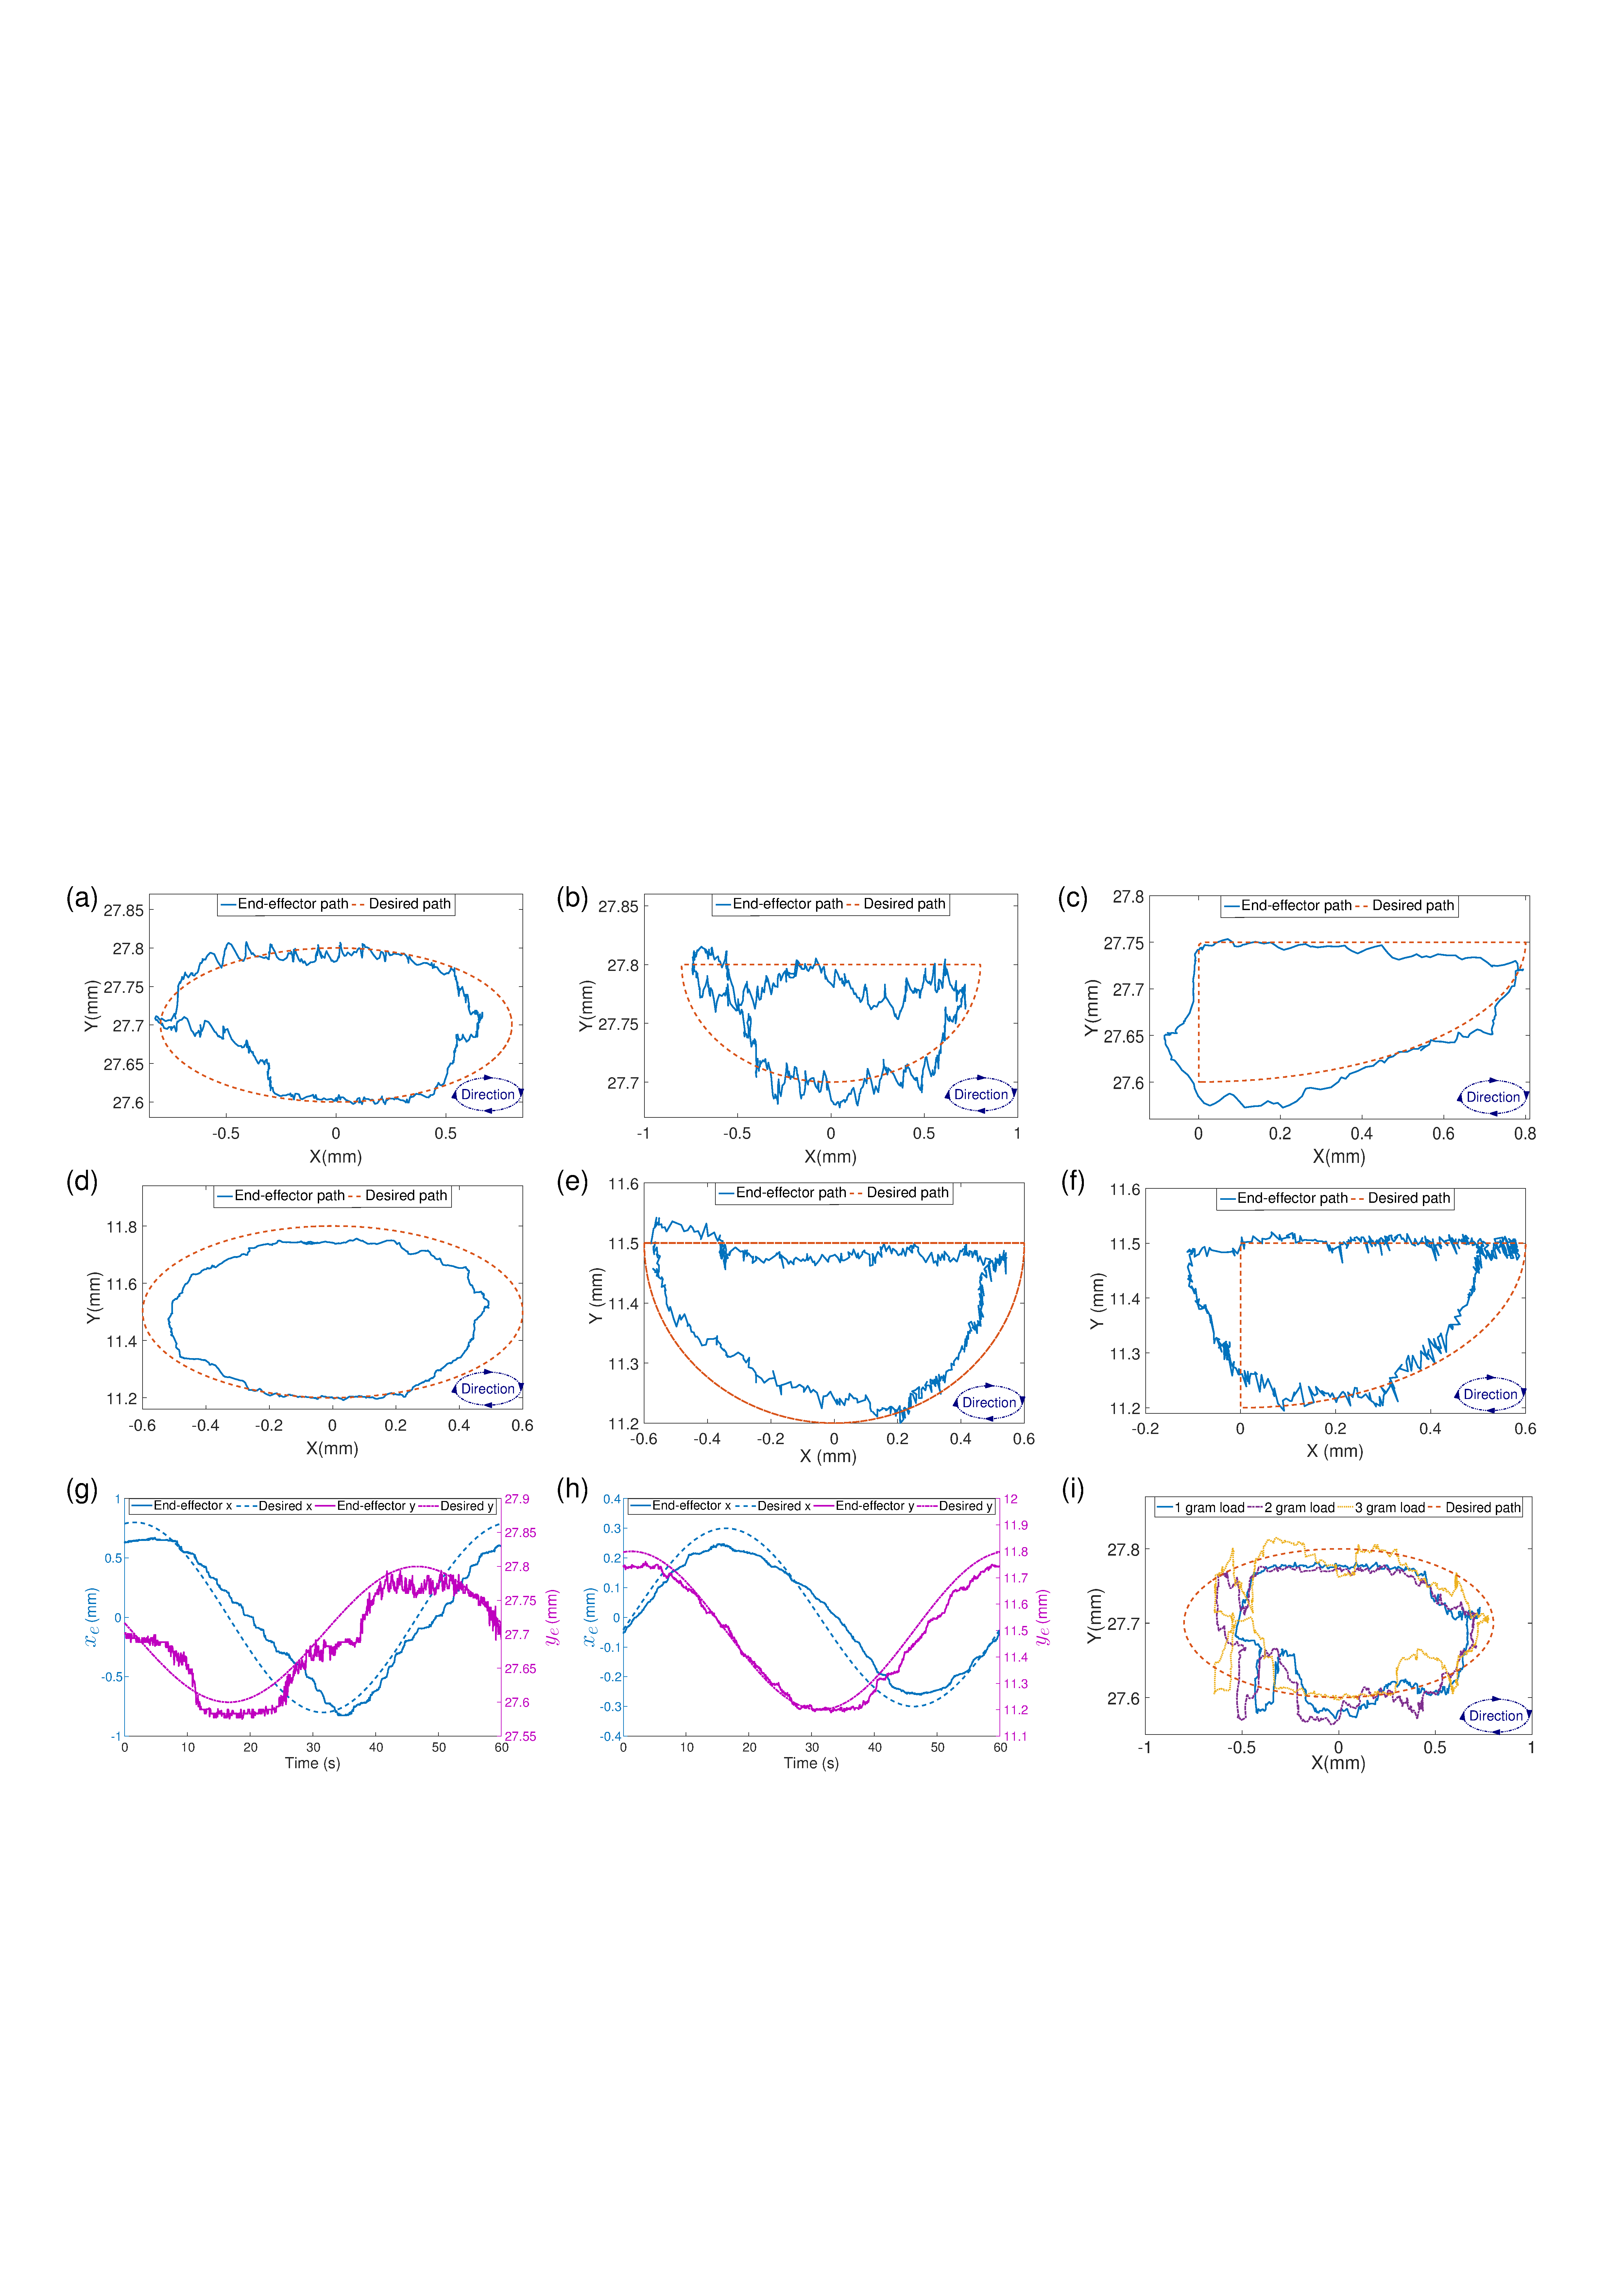
\includegraphics[width=\textwidth]{Control_Picture_New_Ten.pdf}
    \caption[\capitalisewords{Tracking reference and experimental trajectories of  manipulator tip}]{Tracking reference and experimental trajectories of  manipulator tip in Cartesian coordinates. 25\,mm manipulator tracking: (a) an elliptical trajectory; (b) a half-ellipse; (c) a quarter-ellipse. 9\,mm manipulator tracking: (d) an elliptical trajectory; (e) a half-ellipse; (f) a quarter-ellipse. (g) 25\,mm manipulator tracking an elliptical trajectory: $x,y$ coordinates over time separately. (h) 9\,mm manipulator tracking an elliptical trajectory: $x,y$ coordinates over time separately. (i) 25\,mm manipulator tracking an elliptical trajectory under 1\,g, 2\,g, and 3\,g.}
    \label{fig:Control_outputs}
\end{figure*}


Figure~\ref{fig:Control_outputs}a compares the trajectory of a manipulator with the 25\,mm extension driven by the controller Equation~\eqref{eq:Hinf-ctl} along an elliptical reference trajectory. Controller performance was evaluated using a half-ellipse and quarter-ellipse reference trajectory as well, to verify the ability of the controlled system to track straight lines and sharp turns (Figs.~\ref{fig:Control_outputs}b and~\ref{fig:Control_outputs}c). Figures~\ref{fig:Control_outputs}d, ~\ref{fig:Control_outputs}e ,and~\ref{fig:Control_outputs}f show the controlled position of the 9\,mm extension's tip using the same reference trajectories. Figures~\ref{fig:Control_outputs}g and~\ref{fig:Control_outputs}h illustrate the time evolution of the $x$ and $y$ coordinates separately for the two extensions.

\begin{table}[t]
\centering
\caption{(N)MAE of $H_{\infty}$ controller performance in experiment.}\vspace{-0.25cm}
\begin{tabular}{c c c c c c c}
\hline
\hspace{-2mm} $d$ & Reference & Load & $x$ & $y$ & $x-y$ & \hspace{-2mm} NMAE\\
\hspace{-2mm} (mm) &  trajectory   & (g)  & (mm)& (mm)& (mm) & \hspace{-2mm}$\%$\\
\hline
\hspace{-2mm}25 & Ellipse          & - & 0.123 & 0.042 & 0.131 & \hspace{-2mm}8.1\\
\hspace{-2mm}25 & Half Ellipse     & - & 0.119 & 0.023 & 0.123 & \hspace{-2mm}7.6\\
\hspace{-2mm}25 & Quarter Ellipse  & - & 0.112 & 0.026 & 0.119 & \hspace{-2mm}7.4\\
\hspace{-2mm}9 & Ellipse           & - & 0.088 & 0.033 & 0.099 & \hspace{-2mm}7.4\\
\hspace{-2mm}9 & Half Ellipse      & - & 0.129 & 0.058 & 0.132 & \hspace{-2mm}9.8\\
\hspace{-2mm}9 & Quarter Ellipse   & - & 0.161 & 0.061 & 0.171 & \hspace{-2mm}12.8\\
\hspace{-2mm}25 & Ellipse          & 1 & 0.140 & 0.022 & 0.144 & \hspace{-2mm}8.9\\
\hspace{-2mm}25 & Ellipse          & 2 & 0.162 & 0.021 & 0.162 & \hspace{-2mm}10.1\\
\hspace{-2mm}25 & Ellipse          & 3 & 0.164 & 0.022 & 0.164 & \hspace{-2mm}10.2\\ 
\hline
\end{tabular}
\label{table:control}
\vspace{-4mm}
\end{table}

%-----------------------------------
\begin{figure*}[t]
\centering
{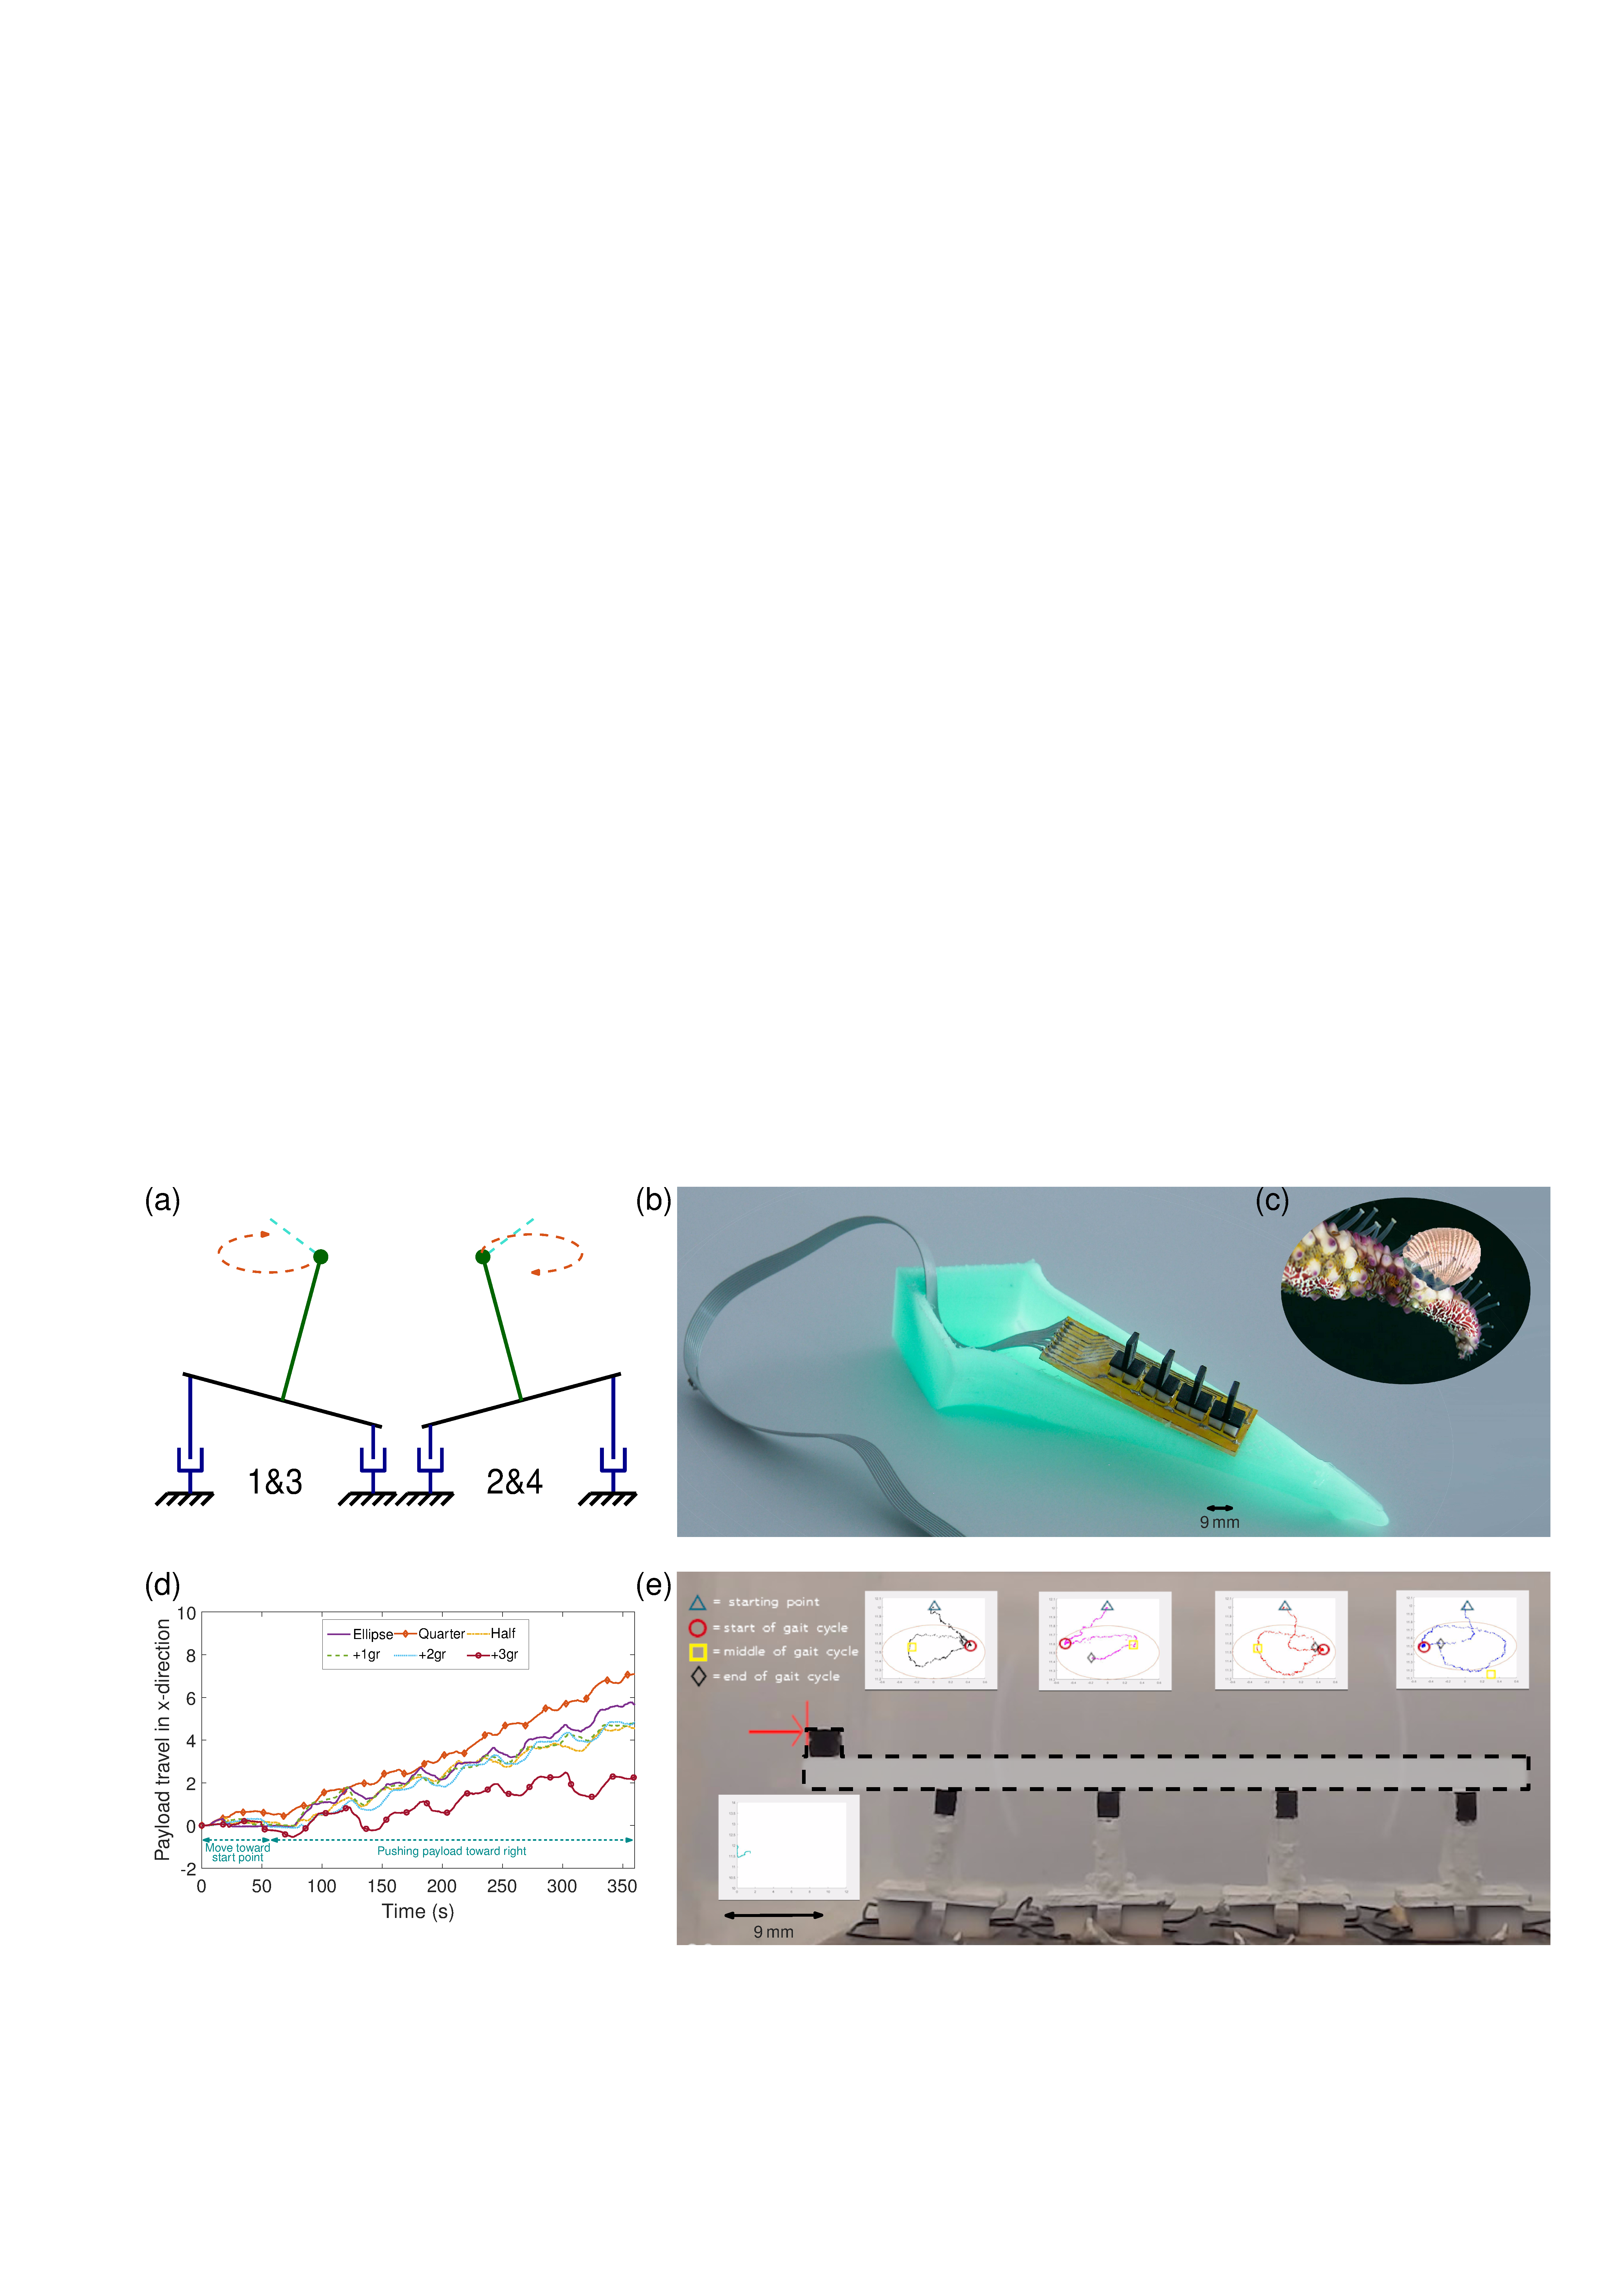
\includegraphics[width=\textwidth]{Starfish_tube_feet_application_8.pdf}}
\caption[\capitalisewords{Control of four 9\,mm manipulators in series for payload transport}]{Control of four 9\,mm manipulators in series for payload transport, in a manner similar to food transport by starfish tube feet. (a) The manipulators, numbered 1 to 4 from left to right, are commanded to first follow the cyan dashed lines from their initial positions to their starting positions on the reference trajectories, and then follow these  trajectories, shown as red dashed lines. Manipulators 1 and 3 have a phase shift of $180^\circ$ compared to manipulators 2 and 4. (b) Illustration of a starfish-inspired robotic platform with four hydrogel-actuated manipulators. (c) Real starfish transporting a clam on its tube feet. (d) Displacement of the payload as a function of time for different reference trajectories and load weights. (e) Array of four manipulators functioning as described in (a) to transport the payload. Image was taken when the manipulators completed the first gait cycle. The payload is a clear flat acrylic plate with a black square on its left side. The positions of the manipulator tips are marked by triangles at their initial locations, circles at the start of the gait cycle, squares at the middle of the gait cycle, and diamonds at the end of the gait cycle.
}
    \label{fig:Control_payload}
\end{figure*}
In order to further characterize our system's actuation capabilities, the manipulator's trajectory-tracking performance under load was studied, as shown in Fig.~\ref{fig:Control_outputs}i. Loads (stainless steel nuts) weighing 1\,g, 2\,g, and 3\,g were placed on the 25\,mm extension, as shown in Fig.~\ref{fig:Path}b. The manipulator was commanded to follow the same elliptical trajectory as in the unloaded case. The results show that the addition of a weight of up to 3\,g increases the trajectory tracking NMAE from 8.1$\%$ to 10.2$\%$ (see Table~\ref{table:control}). Despite the increase in error, each actuator is still able to function under a load as large as 12.5 times its own weight (0.12\,g).
% Tracking the given trajectories requires each SVA to cycle through multiple phases of heating and cooling. As can be observed in Fig.~\ref{fig:Control_outputs}, tracking error is evident for each reference trajectory.The largest tracking error in all cases occurs along a portion of the trajectory in the lower left quadrant of the plots, in which, both SVAs are cooling. Accounting for the different time-constants of the SVAs in heating and cooling states, this transition is not well-characterized in our model obtained by black-box system identification, which results in less accurate trajectory tracking along this portion. We believe, therefore, that the largest difference between our simulated and experimental results can be attributed to the model's inability to characterize the state of SVA heating or cooling. 
As shown in Table~\ref{table:control}, the experimental NMAE values are higher than the simulation values, but remain below $15$\%.


\subsubsection{Payload transport application} \label{sec:payload}
Inspired by the way starfish transport food using their tube feet (Figs.~\ref{fig:Control_payload}b and~\ref{fig:Control_payload}c)~\cite{Kerkut1953,Pentreath1970}, we configured an array of four 9\,mm manipulators, as shown in Fig.~\ref{fig:Control_payload}e, and applied the proposed $H_\infty$-optimal controller in~\eqref{eq:Hinf-ctl} and Fig.~\ref{fig:control_block}b to each manipulator in order to transport a payload across their tips. The payload being transported is a clear acrylic plate. The manipulators are commanded to track reference trajectories as depicted in Fig.~\ref{fig:Control_payload}a, with phase shifts between adjacent manipulators. The payload moves to the right as the manipulators complete repeated cycles of the reference trajectories (``gait cycles''), as shown in Figs.~\ref{fig:Control_payload}d and~\ref{fig:Control_payload}e. The data from Fig.~\ref{fig:Control_payload}d on the duration of one gait cycle and the payload displacement in each tested scenario including the ones with extra added loads on the payload are reported in Table~\ref{table:table_Payload displacement}. A video of the payload transport is attached as supplementary material. The payload's position is recorded but not controlled in this exemplar application, since our goal in this chapter was to demonstrate a use-case for trajectory tracking control. However, many other platforms and applications are possible, including bio-inspired ones~\cite{Doroudchi2020}. Through this example, we have demonstrated how trajectory tracking control of systems with soft actuators, when applied to even simple platforms such as this 2-DOF manipulator, may be used to complete complex tasks such as object transport when used in parallel. This type of design can be used to simplify and decouple the control structures in future applications to reduce computational expense.

\begin{table}[t]
\centering
\caption{Payload displacement $\Delta X$ with different reference trajectories for the manipulators.}
\label{table:table_Payload displacement}
\begin{tabular}{c c c c}

% & & \\ 
\hline
Reference & Payload weight & Time for one & $\Delta X$ after five \\
trajectory & + load (g) & gait cycle (s) & gait cycles (mm)\\
\hline
Ellipse         & 2.7   & 60  & 5.66\\
Half-ellipse    & 2.7   & 50  & 4.55\\
Quarter-ellipse & 2.7   & 40  & 7.10\\
Ellipse         & 2.7+1 & 60  & 4.75\\
Ellipse         & 2.7+2 & 60  & 4.84\\
Ellipse         & 2.7+3 & 60  & 2.30\\
% Open-loop  & 2.7~g & N/A & 2.04~mm\\
\hline
\end{tabular}
\end{table}

\section{\capitalisewords{Conclusions}}
We have shown that the voxel-based design and manufacturing strategy, combined with an electrically addressable smart material, can lead to the creation of miniaturized soft robots with a high number of DOFs. These robots can be used for tasks in which redundancy is needed for example to handle continuously changing tasks in unstructured environments. This has been demonstrated through a miniaturized hyper-redundant soft robot with 16 SVA units.
SVAs can be easily integrated into robotic systems. They help greatly reduce the size of the robots. In addition, sice the SVAs are electrically controlled, they can be connected directly to small footprint microcontrollers and other electronics. The electronics and power supply can be embedded in the robot  and cut the tether from the entire system. We have demonstrated this through a miniature underwater walking robot that do not rely on external signals or power which can be beneficial in applications such as under water data collection and ocean monitoring. The SVAs introduced in Chapter~\ref{chap:SVAs} are the first demonstration of active, soft voxels that are made of stimuli-responsive materials. Using SVAs as building blocks offers higher number of design parameters, namely, the configuration of the SVAs, the material properties of each SVA, and the activation voltage of each SVA. Multi-objective optimization can be used in future to optimize this rich set of design parameters to build structures that have higher force production capacity and %higher 
energy efficiency.
% miniature and micro-scale soft actuators have matured more slowly than their  macro-scale counterparts. 

